% $Id$
% ---------------------------------------------------------------------------
%
%  This is part of the SIGI.
%  Copyright (C) 2008 Interlegis
%  See the file relatorio.tex for copying conditions.
%

\section{Casos de Uso}
\label{sec:casos}

Esta seção descreve a utilização do sistema através de \emph{Casos de
  Uso}, representando os principais atores e suas interações com o
sistema.

Os Casos de Uso serve de auxílio à compreensão, por parte dos
usuários, de como o sistema tende a ser implementado e como é
pretendido que o mesmo venha a ser utilizado.

\subsection{Casos de Uso do SIGI}
Na Figura \ref{fig:casos} temos os Casos de Uso do SIGI de maneira
simplificada.

\begin{figure}[h]
  \centering
  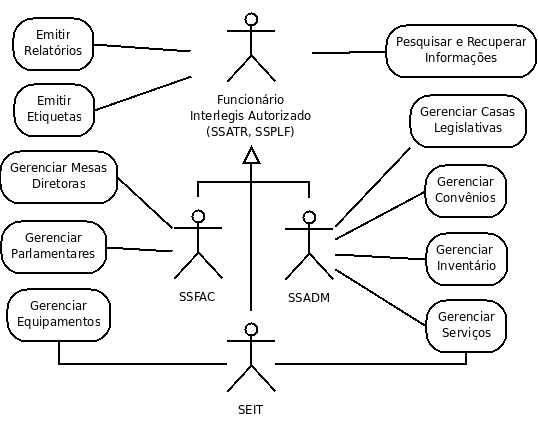
\includegraphics[width=120mm]{../imagens/casosdeuso.png}
  \caption{Casos de uso}
  \label{fig:casos}
\end{figure}

\subsubsection{Descrição dos Atores}
\begin{description}
\item[Funcionário Interlegis:] usuário apenas com atribuições de
  leitura no sistema.
\item[Responsável pela Comunicação:] usuário da Subsecretaria de
  Formação e Atendimento à Comunidade do Legislativo (SSFAC).
\item[Responsável pelo Convênio:] usuário do Serviço de Contratos e
  Convênios (SCCO).
\item[Responsável pela Infra-estrutura:] usuário do Serviço de
  Infra-estrutura Tecnológica (SEIT).
\end{description}

\subsubsection{Descrição das Atividades}
\begin{description}
\item[Emitir Relatórios:] consiste em obter informações e emitir
  relatórios de diversas partes do sistema.
\item[Emitir Etiquetas:] consiste em obter informações e emitir
  etiquetas de algumas partes do sistema.
\item[Gerenciar Mesas Diretoras:] consiste em inserir, atualizar e
  remover \emph{Mesas Diretoras}, \emph{Sessões Legislativas} e
  modificar a \emph{Composição das Mesas Diretoras}.
\item[Gerenciar Parlamentares:] consiste em inserir, atualizar e
  remover \emph{Parlamentares} e \emph{Partidos}.
\item[Gerenciar Equipamentos:] consiste em inserir, atualizar e
  remover \emph{Equipamentos} e \emph{Fornecedores}.
\item[Gerenciar Casas Legislativas:] consiste em inserir, atualizar e
  remover \emph{Casas Legislativas}.
\item[Gerenciar Convênios:] consiste em inserir, atualizar e remover
  \emph{Convênios}.
\item[Gerenciar Inventário:] consiste em atualizar o \emph{Inventário}
  das Casas Legislativas.
\item[Gerenciar Serviços:] consiste em inserir, atualizar e remover
  \emph{Serviços} prestados às Casas Legislativas.
\end{description}

%
% Local variables:
%   mode: flyspell
%   TeX-master: "relatorio.tex"
% End:
%
